\section{Methodology}
\label{sec:method}

We design a three-stage pipeline: (1)~scenario and variant construction, (2)~perplexity measurement, and (3)~introspection probing. \Figref{fig:method_overview} illustrates the overall approach.

\begin{figure}[t]
    \centering
    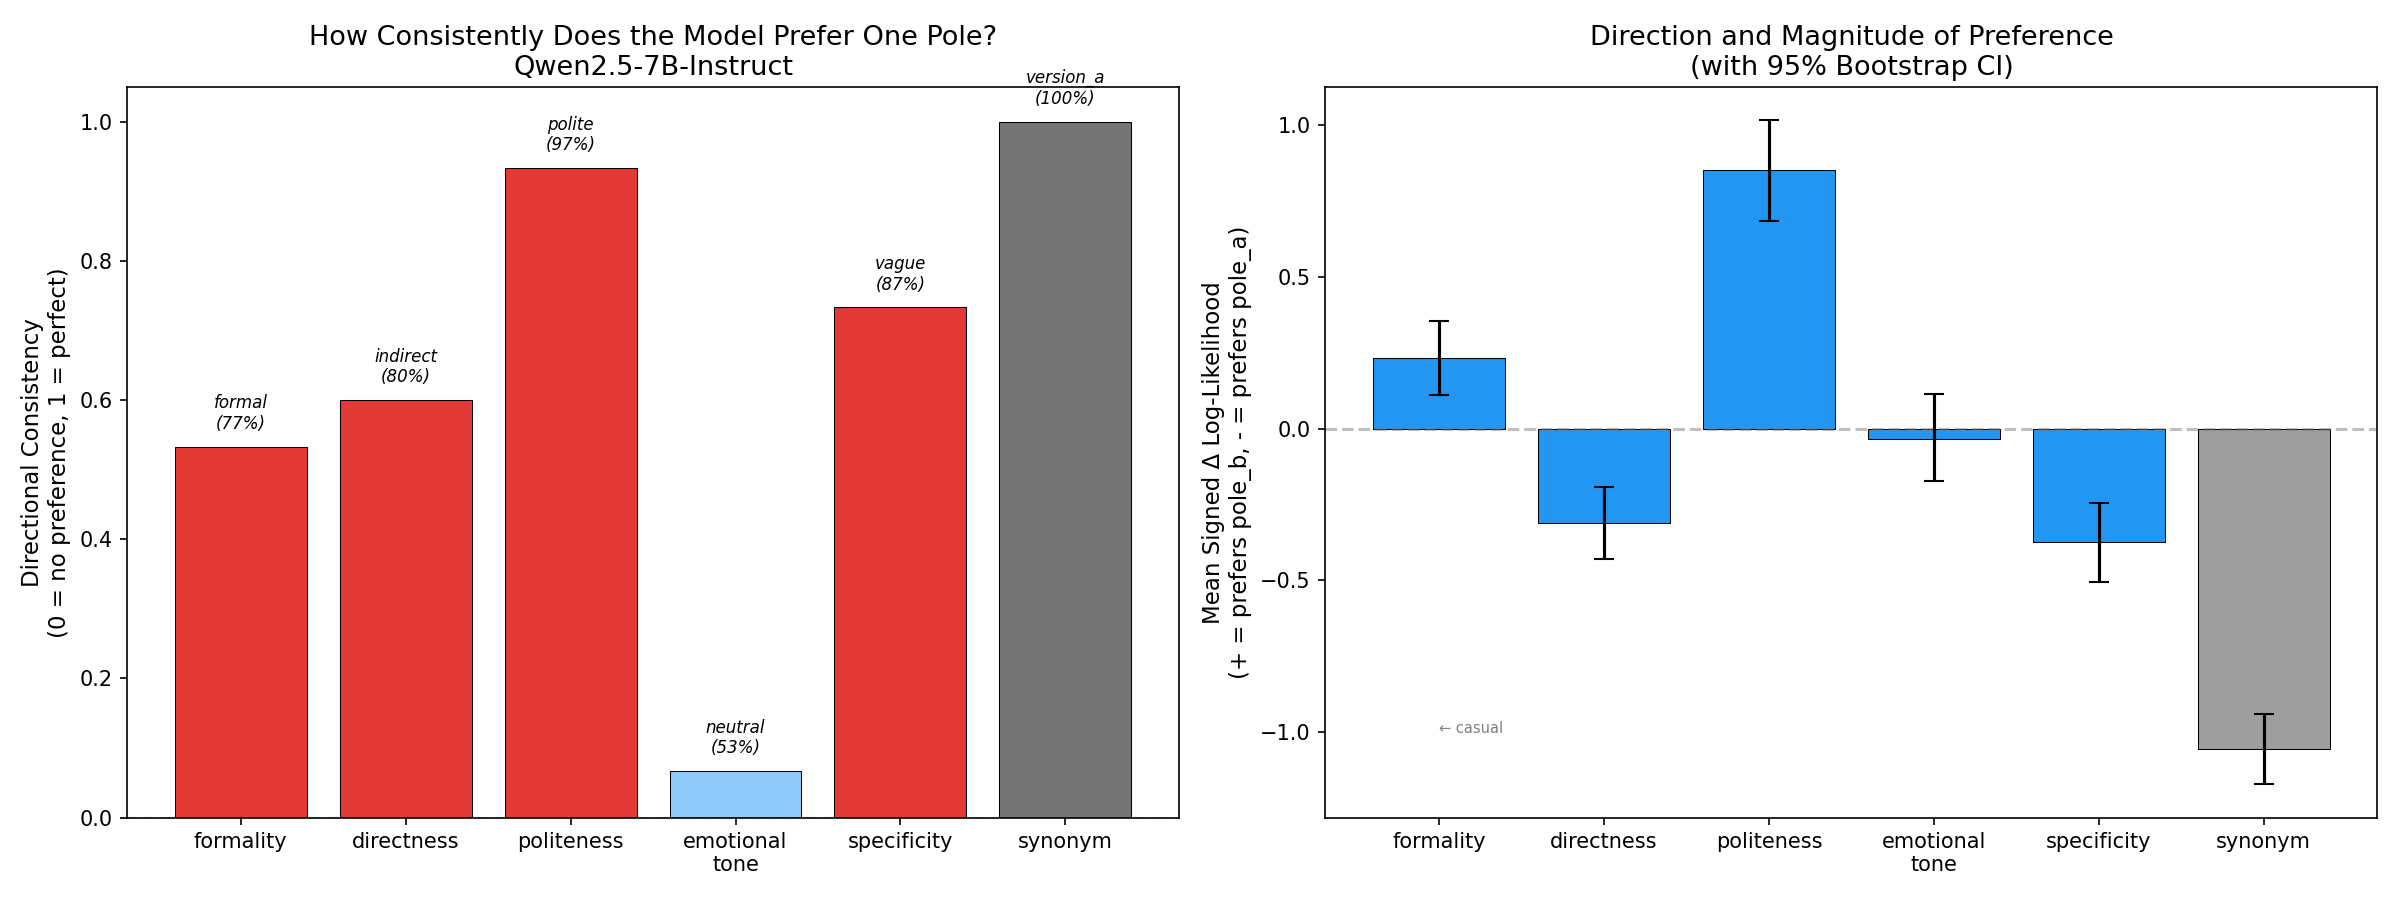
\includegraphics[width=0.95\linewidth]{figures/directional_preferences.png}
    \caption{Directional preferences across pragmatic axes for \qwenseven. \figleft Bar heights show the percentage of scenarios in which the model prefers each pole. \figright Mean signed log-likelihood difference ($\dloglik$) per axis. Politeness shows the strongest directional preference (96.7\% prefer polite), while emotional tone is near chance (46.7\%).}
    \label{fig:method_overview}
\end{figure}

\subsection{Scenario and Variant Construction}
\label{sec:scenarios}

We use \gptfour to generate 30 diverse message-writing scenarios across three communicative domains (10 each):
\begin{itemize}[leftmargin=*,itemsep=0pt,topsep=0pt]
    \item \textbf{Workplace}: emails to a boss, colleagues, clients, or HR
    \item \textbf{Personal}: messages to friends, family, or neighbors
    \item \textbf{Service}: complaints, requests, feedback, or applications
\end{itemize}

For each scenario, we generate response pairs along six axes: five pragmatic axes and one control. Each pair is constrained to differ primarily on the target axis, with matched length (${\leq}20\%$ difference). \Tabref{tab:axes} defines the axes and their poles.

\begin{table}[t]
    \centering
    \caption{Pragmatic axes tested in our experiments. Each axis defines two poles; response pairs are generated to differ primarily along the target axis. The synonym control tests sensitivity to surface-level word choice.}
    \begin{tabular}{@{}llll@{}}
        \toprule
        \textbf{Axis} & \textbf{Pole A} & \textbf{Pole B} & \textbf{Type} \\
        \midrule
        Formality & casual / informal & formal / professional & pragmatic \\
        Directness & indirect / hedged & direct / assertive & pragmatic \\
        Politeness & blunt / terse & polite / courteous & pragmatic \\
        Emotional tone & neutral / factual & warm / empathetic & pragmatic \\
        Specificity & vague / general & detailed / specific & pragmatic \\
        \midrule
        Synonym & version A & version B & control \\
        \bottomrule
    \end{tabular}
    \label{tab:axes}
\end{table}

This yields $30 \times 6 = 180$ variant pairs. All scenario and variant generation uses \gptfour with temperature 0.7--0.8.

\subsection{Perplexity Measurement}
\label{sec:perplexity}

For each prompt--response pair $(p, r)$, we compute the conditional log-likelihood of the response given the prompt:
\begin{equation}
    \loglik(r \mid p) = \frac{1}{|r|} \sum_{t=1}^{|r|} \log P_\theta(r_t \mid p, r_{<t})
    \label{eq:loglik}
\end{equation}
where $|r|$ is the number of response tokens, $r_t$ is the $t$-th token, and $P_\theta$ is the model's next-token distribution. We tokenize using the model's chat template to match the format seen during training.

For each scenario $s$ and axis $a$, we compute the \emph{signed difference}:
\begin{equation}
    \dloglik_{s,a} = \loglik(r^{(b)}_{s,a} \mid p_s) - \loglik(r^{(a)}_{s,a} \mid p_s)
    \label{eq:delta}
\end{equation}
where $r^{(a)}$ and $r^{(b)}$ are the Pole~A and Pole~B responses, respectively. A positive $\dloglik$ indicates the model prefers Pole~B; a negative value indicates preference for Pole~A.

\subsection{Introspection Probing}
\label{sec:introspection}

To compare behavioral detection against self-report, we prompt \gptfour (temperature 0.3) to generate a response for each scenario and simultaneously list all pragmatic variables it considered. We then map self-reported variables to our five axes using keyword matching (\eg mentions of ``tone,'' ``empathy,'' or ``warmth'' map to emotional tone).

Note that introspection is measured on \gptfour rather than the Qwen models used for perplexity, because the Qwen models at 3B--7B parameters do not produce reliable introspective reports. This design choice means our behavioral--introspective comparison is cross-model; we discuss the implications in \secref{sec:limitations}.

\subsection{Statistical Analysis}
\label{sec:stats}

For each axis, we test whether $\dloglik$ differs from zero across 30 scenarios using:
\begin{itemize}[leftmargin=*,itemsep=0pt,topsep=0pt]
    \item \textbf{Wilcoxon signed-rank test}: non-parametric test for location shift
    \item \textbf{Sign test} (exact binomial): whether directional preference exceeds 50\%
    \item \textbf{Cohen's $d$}: effect size of the signed differences from zero
    \item \textbf{Bootstrap 95\% CI}: 10{,}000 resamples of the mean $\dloglik$
\end{itemize}

We apply Bonferroni correction for six comparisons ($\alpha = 0.05/6 \approx 0.0083$). We define \emph{directional consistency} as $|2f - 1|$ where $f$ is the fraction of scenarios preferring the majority pole, yielding values from 0 (no preference) to 1 (unanimous).

\subsection{Models}
\label{sec:models}

\begin{table}[t]
    \centering
    \caption{Models used in our experiments.}
    \begin{tabular}{@{}llr@{}}
        \toprule
        \textbf{Model} & \textbf{Role} & \textbf{Parameters} \\
        \midrule
        \qwenseven & primary perplexity probe & 7.6B \\
        \qwenthree & cross-size replication & 3.1B \\
        \gptfour & scenario generation, introspection & --- \\
        \bottomrule
    \end{tabular}
    \label{tab:models}
\end{table}

\Tabref{tab:models} summarizes our models. The Qwen models run locally on NVIDIA RTX A6000 GPUs with CUDA~12.5, PyTorch~2.5.1, and Transformers~5.5.0. All experiments use a fixed random seed of 42.
